\documentclass{classrep}
\usepackage[utf8]{inputenc}
\usepackage{color}
\usepackage{enumitem}
\usepackage{graphicx}
\usepackage{amsmath}
\usepackage{float}


\studycycle{Informatyka, studia dzienne, I st.}
\coursesemester{VI}

\coursename{Komputerowe systemy rozpoznawania}
\courseyear{2019/2020}

\courseteacher{dr hab. inż. Adam Niewiadomski prof. uczelni}
\coursegroup{pon., 12:15}

\author{
\studentinfo{Mateusz Walczak}{216911} \and
\studentinfo{Konrad Kajszczak}{216790}
}

\title{Zadanie 1: Ekstrakcja cech, miary podobieństwa, klasyfikacja}
\svnurl{https://github.com/Walducha1908/KSR1}

\begin{document}
\maketitle

\section{Cel}
{Celem zadania było stworzenie aplikacji służącej do klasyfikacji artykułów prasowych metodą k-NN. Korzystając z różnych metod
wyboru słów kluczowych i ekstrakcji wektorów cech oraz istniejących miar podobieństwa, należało porównać przypisane przez naszą aplikacje kategorie artykułów do tych faktycznych. Należało również podjąć próbę opracowania własnej miary podobieństwa i/lub metryki.}

\section{Wprowadzenie}
 Algorytm k najbliższych sąsiadów jest bardzo prostym klasyfikatorem probabilistycznym. Niekiedy mówi się, że algorytm k-NN jest leniwy. Wynika to z faktu, że nie tworzy on wewnętrznej reprezentacji danych treningowych (uczących), ale ropoczyna poszukiwanie rozwiązania dopiero podczas analizy konkretnego wzorca ze zbioru testowego. \newline

Algorytm przechowuje zbiór wszystkich wzorców uczących, względem których obliczana jest odległość wzorca testowego, zdefiniowana poprzez odpowiednią metrykę. Następnie algorytm wybiera k wzorców treningowych, nazywanych sąsiadami, do których aktualnie badany wzorzec testowy ma najmniejszą odległość. Ostateczny rezultat - kategoria, do której zostanie przypisany analizowany wzorzec - stanowi najczęściej występująca kategoria wśród k najbliższych sąsiadów.

\subsection{Metryki}

Do obliczenia odległości pomiędzy tekstami posłużyliśmy się następującymi metrykami:

\begin{itemize}[label=$\bullet$\scshape\bfseries]

\item Metryka Euklidesowa - w celu obliczenia odległości $ d_{e}(x,y) $ między dwoma punktami $ x, y $ należy obliczyć pierwiastek kwadratowy z sumy kwadratów różnic wartości współrzędnych o tych samych indeksach, zgodnie ze wzorem:
\begin{equation}
d_{e}(x,y)= \sqrt{ (y_{1} - x_{1})^2 + \cdots + (y_{n} - x_{n})^2 }
\end{equation}

\item Metryka uliczna (Manhattan, miejska) - w celu obliczenia odległości $ d_{m}(x,y) $ między dwoma punktami $ x, y $ należy obliczyć sumę wartości bezwzględnych różnic współrzędnych punktów $ x $ oraz $ y $, zgodnie ze wzorem:
\begin{equation}
d_{m}(x,y)= \sum_{k=1}^{n} | x_{k} - y_{k} |
\end{equation}

\item Metryka Czebyszewa - w celu obliczenia odległości $ d_{ch}(x,y) $ między dwoma punktami $ x, y $ należy obliczyć maksymalną wartość bezwzględnych różnic współrzędnych punktów $ x $ oraz $ y $, zgodnie ze wzorem:
\begin{equation}
d_{ch}(x,y)= \max_{i} |x_{i} - y_{i}|
\end{equation}

\item Metryka Hamminga - definiujemy jako ilość różnic pomiędzy dwoma wektorami o tej samej długości. Aby obliczyć odległość $ d_{h}(x,y) $ między dwoma punktami $ x, y $ należy posłużyć się wzorem \cite{wyklad} :
\begin{equation}
d_{h}(x,y)= \sum_{i=1}^{n} |h(i)|,
\end{equation}
gdzie 
\begin{equation}
h(i)= \left\{ \begin{array}{ll}
0 & \textrm{jeśli $v_{1i}=v_{2i}$}\\
1 & \textrm{w przeciwnym wypadku}
\end{array} \right.
\end{equation}

\item Odległość Canberra - ważona wersja metryki ulicznej, aby obliczyć odległość $ d_{c}(x,y) $ między dwoma punktami $ x, y $ należy posłużyć się wzorem:
\begin{equation}
d_{c}(x,y)= \sum_{i} \frac{|x_{i} - y_{i}|}{|x_{i}| + |y_{i}|}
\end{equation}

\end{itemize}

\subsection{Wyznaczanie słów kluczowych}

Aby wyznaczyć słowa kluczowe posługujemy się poniższą metodą:

\begin{itemize}[label=$\bullet$\scshape\bfseries]
\item Term frequency - metoda polegająca na zliczeniu liczby wystąpień danego słowa we wszystkich dokumentach.
\end{itemize}

Przeprowadzamy obliczenia na zbiorze wszystkich posiadanych danych (w naszym przypadku na wszystkich artykułach) i otrzymujemy zestaw par - słowo i wartość. Taki zestaw par sortujemy malejąco po wartości i wybieramy n pierwszych słów. Wybrane n słów staje się słowami kluczowymi. \newline

Taki schemat powtarzamy $l$ razy, gdzie $l$ jest liczbą kategorii na jakie klasyfikujemy. Ostatecznie otrzymujemy $l$ zestawów słów kluczowych, przy czym każdy zestaw reprezentuje inną kategorię. Otrzymane zbiory słów kluczowych oznaczamy:

\begin{equation}
            K_{1}, K_{2}, \ldots , K_{l-1}, K_{l}.
 \end{equation}	

Otrzymany zbiór słów kluczowych będziemy używać we wszystkich iteracjach programu. Słowa kluczowe będą niezmienne, a wszystkie przeprowadzone przez nas eksperymenty będą bazowały na tym samym zbiorze słów kluczowych.

\subsection{Wyznaczanie ważonych słów kluczowych}

W celach poprawienia jakości klasyfikacji wprowadzono "ważone słowa kluczowe". Tak nazwaliśmy zestaw par - słowo kluczowe i waga (wartość zmiennoprzecinkowa), z wykorzytsaniem których przeprowadziliśmy takie same eksperymenty jak z wykorzystaniem "zwykłych" słów kluczowych, opisanych w poprzednim podpunkcie. \newline

Ważone słowa kluczowe to nic innego jak obliczony wcześniej, ten sam zestaw słów, jednak ubogacony o wagę, obliczaną zgodnie z opracowanym przez nas wzorem:
\begin{equation}
            W_{i} = \left({1 - \frac{N_{W_{i} \in K_{l}}}{l - 1}}\right)^2,
 \end{equation}	

gdzie $W_{i}$ - waga $i$-tego słowa kluczowego, $l$ - liczba kategorii, $N_{W_{i} \in K_{l}}$ - liczba kategorii słów kluczowych (innych od swojej własnej), w których $i$-te słowo kluczowe występuje. \newline

Dla jasności przeanalizujemy przykład. Niech $l = 3$, a obliczone słowa kluczowe mają postać:\newline
\begin{equation}
            K_{1} = \{{"jesien", "ogon", "krowa"}\},
\end{equation}
\begin{equation}
            K_{2} =\{{"wiosna", "ogon", "pies"}\},
\end{equation}	
\begin{equation}
            K_{3} = \{{"lato", "ogon", "krowa"}\},
\end{equation}	

Obliczmy wartości wag dla wybranych słów kluczowych z powyższego zestawu. Dla słowa "jesien" otrzymamy następującą wartość:
\begin{equation}
            W_{jesien} = \left({1 - \frac{0}{2}}\right)^2 = 1,
\end{equation}
słowo "jesien" wystąpiło tylko w jednej, "swojej" kategorii, ma zatem najwiekszą możliwą wagę.

Dla słowa "krowa":
\begin{equation}
            W_{krowa} = \left({1 - \frac{1}{2}}\right)^2 = 0.25,
\end{equation}
słowo "krowa" wystąpiło w jednej dodatkowej kategorii (łącznie w dwóch).

Dla słowa "ogon":
\begin{equation}
            W_{ogon} = \left({1 - \frac{2}{2}}\right)^2 = 0,
\end{equation}
słowo "ogon" wystąpiło we wszystkich kategoriach, dlatego też uznajemy, że nie ma dla nas żadnego znaczenia, jego waga jest równa 0. \newline

Z powyższych rozważań bardzo jasno wynika, że wagi słów kluczowych mogą osiągać wartości z przedziału $ \langle0;1\rangle $.


\subsection{Cechy poddawane ekstrakcji}

Ekstrakcja cech charakterystycznych tekstu - w tym celu tworzymy wektor cech, który opisuje tekst (w naszym przypadku artykuł) na podstawie konkretnych, zdefiniowanych cech. Poniżej znajduje się opis wszystkich cech użytych w doświadczeniu. \newline

Przed ekstrakcją cech, tekst został odpowiednio przygotowany. Z artykułów usunięte zostały nic nie wnoszące słowa (z tzw. "stop" listy), tekst został poddany stemizacji oraz pozbawiony znaków interpunkcyjnych. \newline

Przyjęto następujące oznaczenia:\\
    \quad $T_{i}$ - zbiór słów do badania,\\
    \quad $K$ - stały zbiór słów kluczowych\footnote{Na który składają się zbiory ${K_{1}, K_{2}, \ldots , K_{l-1}, K_{l}.}$}, \\
    \quad $N_{K \in T}$ - liczba wystąpień elementów zbioru K w zbiorze T\footnote{W przypadku ważonych słów kluczowych będzie to suma iloczynów liczby wystąpień poszczególnych elementów zbioru K w zbiorze T i odpowiadających im wag.}, \\
    \quad $C_{i}(T,K)$ - wartość funkcji cechy. \\


\subsubsection{Liczba wystąpień wszystkich słów kluczowych w całym artykule}
Cecha opisująca liczbę słów kluczowych, które występują w całej sekcji głównej artykułu (body).
\begin{equation}
            C_{1}(T_{1},K) = N_{K \in T_{1}},
 \end{equation}	
 gdzie $T_{1}$ - zbiór słów sekcji głównej artykułu. \newline

Przeanalizujmy przykład obliczania wartości cechy $C_{1}$. Niech zbiór słów kluczowych $K$ ma postać:
\begin{equation}
K = \{{"wirus", "choroba", "zaraz", "anihilacja"}\},
 \end{equation}	
zaś zbiór słów do badania (zbiór słów sekcji głównej badanego artykułu testowego) $T_{1}$ prezentuje się następująco:
\begin{equation}
\begin{split}
T_{1} = \{{"wirus", "niszczy", "wszystko", "droga",}\\ 
{"zaraz", "wirus", "powodowac", "choroba"}\},
\end{split}
\end{equation}	

Najpierw w wariancie pierwszej metody ekstrakcji - wykorzystując metodę TF i zwykłe słowa kluczowe. Przeanalizujmy występowanie elementów zbioru $K$  w zbiorze $T_{1}$:
\begin{itemize}[label=$\bullet$\scshape\bfseries]
\item "wirus" - występuje 2 razy,
\item "choroba" - występuje 1 raz,
\item "zaraz" - występuje 1 raz,
\item "anihilacja" - nie występuje ani razu.
\end{itemize}

Po dodaniu wszystkich wystąpień otrzymujemy:
\begin{equation}
 C_{1}(T_{1},K) =  N_{K \in T_{1}} = 2+1+1+0= 4.
 \end{equation}	

Teraz zajmijmy się drugą metodą ekstrakcji - wykorzystując ważone słowa kluczowe. Załóżmy, że pary słów kluczowych wraz z obliczonymi wagami dla słów kluczowych zbioru $K$ prezentują się następująco:
\begin{equation}
K_{w} = \{{("wirus", 0.25), ("choroba", 1), ("zaraz", 0), ("anihilacja", 1)}\},
 \end{equation}	

W tym przypadku zgodnie z wcześniej zaprezentowanym opisem, musimy obliczyć sumę iloczynów liczby wystąpień poszczególnych elementów zbioru $K$ w zbiorze $T_{1}$ i odpowiadających im wag:
\begin{equation}
 C_{1}(T_{1},K_{w}) =  N_{K \in T_{1}} = 2 \cdot 0.25 + 1 \cdot 1 + 1 \cdot 0 + 0 \cdot 1 = 0.5 + 1 + 0 + 0 = 1.5.
 \end{equation}	

\subsubsection{Liczba wystąpień wszystkich słów kluczowych w tytule artykułu}
Cecha opisująca liczbę słów kluczowych, które występują w tytule artykułu (title).
\begin{equation}
            C_{2}(T_{2},K) = N_{K \in T_{2}},
 \end{equation}	
 gdzie $T_{2}$ - zbiór słów tytułu artykułu.

\subsubsection{Liczba wystąpień wszystkich słów kluczowych w sekcji daty artykułu}

Cecha opisująca liczbę słów kluczowych, które występują w sekcji daty artykułu (dateline).
\begin{equation}
            C_{3}(T_{3},K) = N_{K \in T_{3}},
 \end{equation}	
 gdzie $T_{3}$ - zbiór słów sekcji daty artykułu.

\subsubsection{Stosunek liczby wystąpień wszystkich słów kluczowych do ogólnej liczby słów w artykule}
Cecha opisująca stosunek liczby słów kluczowych, które występują w całej sekcji głównej artykułu (body), do całkowitej liczby słów występujących w części głównej.
\begin{equation}
            C_{4}(T_{4},K) = \frac{N_{K \in T_{4}}} {|T_{4}|},
 \end{equation}	
 gdzie $T_{4}$ - zbiór słów sekcji głównej artykułu, $|T_{4}|$ - liczba elementów (słów) zbioru sekcji głównej artykułu. \newline

W tym miejscu warto wspomnieć, że w przypadku ważonych słów kluczowych wartość $|T_{4}|$ będzię iloczynem liczby elementów zbioru sekcji głównej artykułu i maksymalnej wartości osiągalnej przez wagi. Jednak ponieważ maksymalną możliwą wartością wagi słowa kluczowego jest 1 (zgodnie z rozdziałem 2.3) to w obu przypadkach - zwykłych słów kluczowych jak i ważonych słów kluczowych - będzie to dokładnie ta sama wartość liczbowa.

\subsubsection{Liczba wystąpień wszystkich słów kluczowych w pierwszych 50 słowach artykułu}
Cecha opisująca liczbę słów kluczowych, które występują w pierwszych 50 słowach sekcji głównej artykułu. Jeśli artykuł jest krótszy niż 50 słów to bierzemy pod uwagę wszystkie występujące w nim słowa.
\begin{equation}
            C_{5}(T_{5},K) = N_{K \in T_{5}},
 \end{equation}	
 gdzie $T_{5}$ - pierwsze 50 słów sekcji głównej artykułu.

\subsubsection {Liczba wystąpień wszystkich słów kluczowych w pierwszych 10\% artykułu}
Cecha opisująca liczbę słów kluczowych, które występują w pierwszych 10\% sekcji głównej artykułu.
\begin{equation}
            C_{6}(T_{6},K) = N_{K \in T_{6}},
 \end{equation}	
 gdzie $T_{6}$ - pierwsze 10\% słów sekcji głównej artykułu.

\subsubsection{Liczba wystąpień wszystkich słów kluczowych w pierwszych 20\% artykułu}
Cecha opisująca liczbę słów kluczowych, które występują w pierwszych 20\% sekcji głównej artykułu.
\begin{equation}
            C_{7}(T_{7},K) = N_{K \in T_{7}},
 \end{equation}	
 gdzie $T_{7}$ - pierwsze 20\% słów sekcji głównej artykułu.

\subsubsection{Liczba wystąpień wszystkich słów kluczowych w pierwszych 50\% artykułu}
Cecha opisująca liczbę słów kluczowych, które występują w pierwszych 50\% sekcji głównej artykułu.
\begin{equation}
            C_{8}(T_{8},K) = N_{K \in T_{8}},
 \end{equation}	
 gdzie $T_{8}$ - pierwsze 50\% słów sekcji głównej artykułu.

\subsubsection{Liczba wystąpień wszystkich słów kluczowych w pierwszym paragrafie}
Cecha opisująca liczbę słów kluczowych, które występują w pierwszym paragrafie sekcji głównej artykułu.
\begin{equation}
            C_{9}(T_{9},K) = N_{K \in T_{9}},
 \end{equation}	
 gdzie $T_{9}$ - pierwszy paragraf sekcji głównej artykułu.

\subsubsection{Liczba wystąpień wszystkich słów kluczowych w ostatnich 50 słowach artykułu}
Cecha opisująca liczbę słów kluczowych, które występują w ostatnich 50 słowach sekcji głównej artykułu. Jeśli artykuł jest krótszy niż 50 słów to bierzemy pod uwagę wszystkie występujące w nim słowa.
\begin{equation}
            C_{10}(T_{10},K) = N_{K \in T_{10}},
 \end{equation}	
 gdzie $T_{10}$ - ostatnie 50 słów sekcji głównej artykułu.

\subsubsection{Liczba wystąpień wszystkich słów kluczowych w ostatnich 10\% artykułu}
Cecha opisująca liczbę słów kluczowych, które występują w ostatnich 10\% sekcji głównej artykułu.
\begin{equation}
            C_{11}(T_{11},K) = N_{K \in T_{11}},
 \end{equation}	
 gdzie $T_{11}$ - ostatnie 10\% słów sekcji głównej artykułu.

\subsubsection{Liczba wystąpień wszystkich słów kluczowych w ostatnim paragrafie}
Cecha opisująca liczbę słów kluczowych, które występują w ostatnim paragrafie sekcji głównej artykułu.
\begin{equation}
            C_{12}(T_{12},K) = N_{K \in T_{12}},
 \end{equation}	
 gdzie $T_{12}$ - ostatni paragraf sekcji głównej artykułu.

\section{Opis implementacji}
Program został napisany w języku Java z wykorzystaniem narzędzia Maven \cite{Maven}, służącego do automatyzacji budowy oprogramowania. \newline

Aplikacja została podzielona na następujące pakiety:
\begin{itemize}[label=$\bullet$\scshape\bfseries]
\item $Data$,
\item $Model$ zawierający podpakiety $Testing$ i $Training$,
\item $Features$,
\item $Calculations$ zawierający podpakiety $KeyWords$, $Features$, $KNN$ i $Metrics$,
\item $Main$.
\end{itemize}

W tym rozdziale omówione zostaną wszystkie wyżej wymienione pakiety. Przedstawimy diagramy UML każdego z pakietów a także omówimy zastosowanie poszczególnych klas.

\subsection{Pakiet Data}
Pakiet $Data$ jest odpowiedzialny za wczytywanie danych oraz za przygotowanie struktury obiektów artykułów. Zajmuje się on także eksportowaniem raportu z wyników badań w formacie $xlsx$.

\begin{figure}[H]
	\centering
	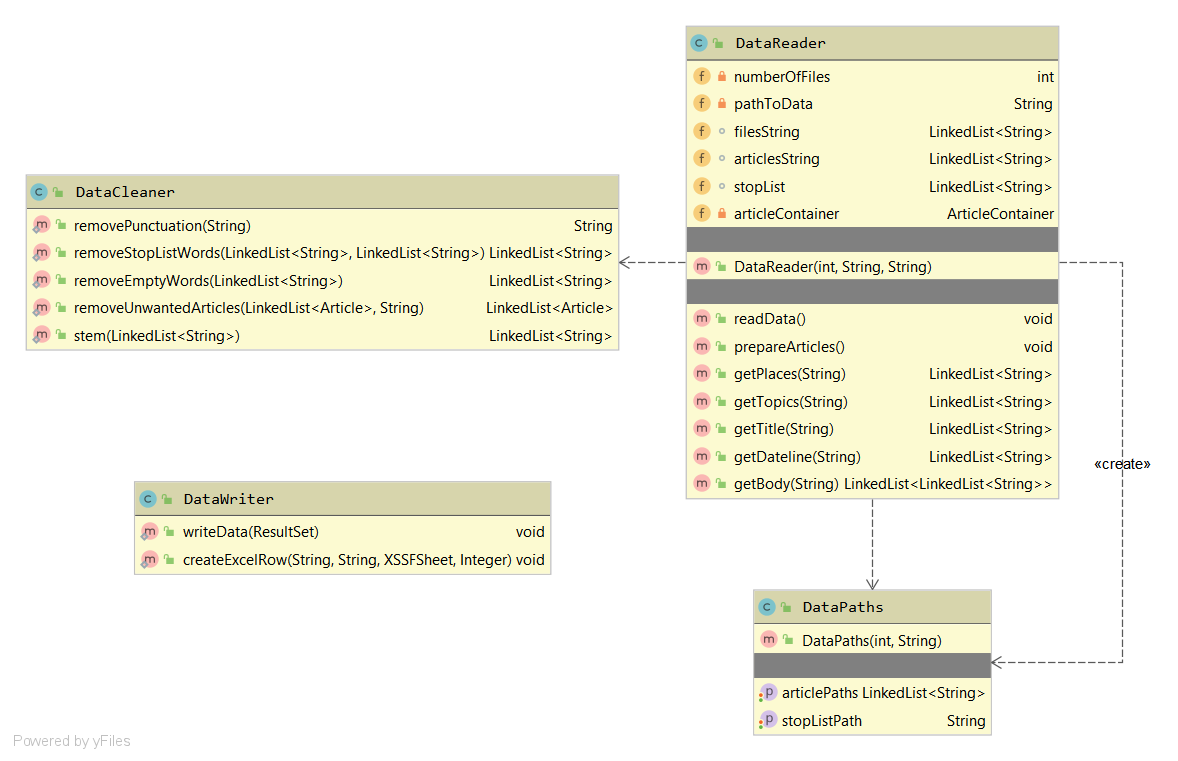
\includegraphics[width=1\textwidth]{{Diagramy/PackageData.png}}
	\caption{Diagram UML dla pakietu $Data$}
\end{figure}

Klasy omawianego pakietu mają następujące zadania:
\begin{itemize}[label=$\bullet$\scshape\bfseries]
\item $DataReader$ - wczytanie danych z plików i zbudowanie struktury obiektów artykułów,
\item $DataPaths$ - wygenerowanie ścieżek do plików, z których dane będą wczytywane przez obiekt klasy $DataReader$,
\item $DataCleaner$ - usuwanie słów z artykułów należących do tzw. "Stop" listy, usuwanie znaków interpunkcyjnych, pustych słów, artykułów nienależącyh do aktualnego zbioru badawczego, a także przeprowadzanie stemizacji tekstu z użyciem biblioteki $snowball-stemmer$ \cite{Stem}.
\item $DataWriter$ - eksportowanie wyników działania programu do raportu w formacie $xslx$ z wykorzystaniem biblioteki $poi-ooxml$ \cite{Excel}.
\end{itemize}

\subsection{Pakiet Model}
Pakiet $Model$ zawiera strukturę klas modelowych i kontenerowych, opisuje klasy artykułów, słów kluczowych oraz zestawu rezultatów wykonanych badań. Wykonuje również niektóre proste operacje logiczne takie jak dzielenie artykułów na zbiory testowy i treningowy czy obliczanie parametrów określających jakość klasyfikacji. Zawiera dwa podpakiety - $Testing$ oraz $Training$, które opisują strukturę klas artykułów odpowiednio testowych i treningowych.

\begin{figure}[H]
	\centering
	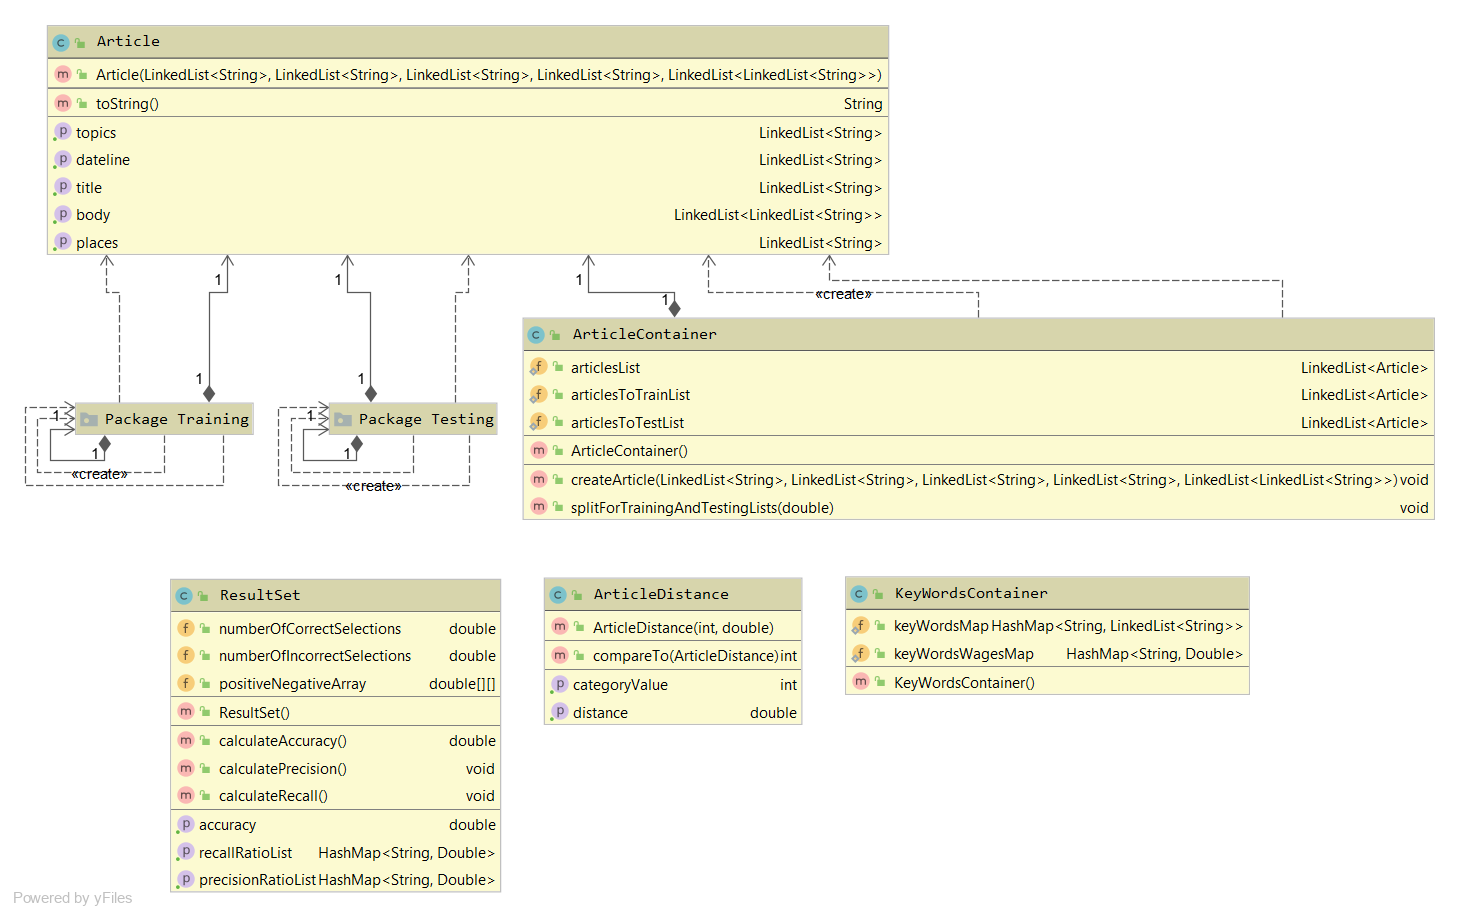
\includegraphics[width=1\textwidth]{{Diagramy/PackageModel.png}}
	\caption{Diagram UML dla pakietu $Model$}
\end{figure}

Klasy pakietu $Model$ są następujące:\newline
\begin{itemize}[label=$\bullet$\scshape\bfseries]
\item $Article$ - klasa modelowa artykułu, przetrzymuje wszystkie listy słów poszczególnych sekcji artykułu,
\item $ArticleContainer$ - klasa kontenerowa przechowująca wszystkie artykuły, dodatkową funkcjonalnością tej klasy jest dzielenie artykułów na testowe i treningowe (w stosunku określonym w klasie $Settings$ w pakiecie $Main$),
\item $ArticleDistance$ - klasa służąca do porównywania odległości pomiędzy artykułami, implmentuje interfejs Comparable,
\item $KeyWordsContainer$ - klasa kontenerowa przechowująca wszystkie słowa kluczowe, w zależności od danej iteracji programu mogą to być zwykłe lub ważone słowa kluczowe,
\item $ResultSet$ - klasa przetrzymująca wyniki przeprowadzonych badań.
\end{itemize}

\subsubsection{Podpakiet Training}
Podpakiet $Training$ zawiera klasy opisujące artykuły treningowe. Obiekt klasy $TrainingArticle$ zostaje utworzony po tym, jak przeprowadzona zostanie pełna ekstrakcja cech dla odpowiadającego mu obiektu klasy $Article$. \newline

Podpakiet $Training$ składa się z dwóch klas:
\begin{itemize}[label=$\bullet$\scshape\bfseries]
\item $TrainingArticle$ - klasa artykułu treningowego zawierająca obiekt klasy $Article$ wraz z wektorem wyekstrahowanych cech,
\item $TrainingArticleContainer$ - klasa kontenerowa przechowująca wszystkie artykuły treningowe (obiekty klasy $TrainingArticle$).
\end{itemize}

\begin{figure}[H]
	\centering
	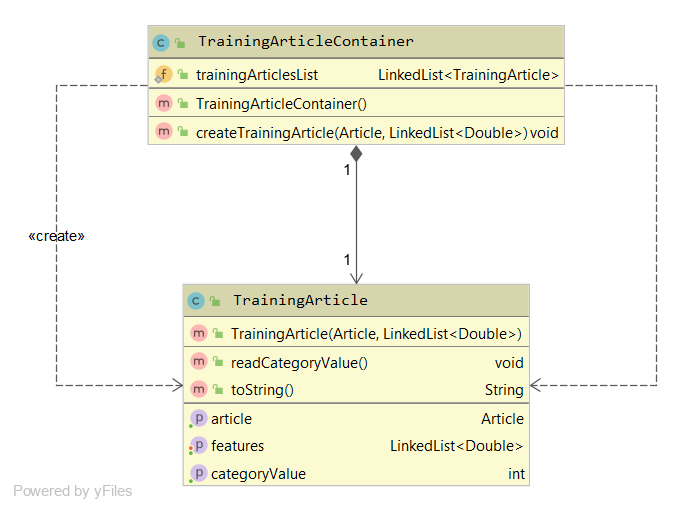
\includegraphics[width=1\textwidth]{{Diagramy/PackageTraining.png}}
	\caption{Diagram UML dla podpakietu $Training$ pakietu $Model$}
\end{figure}

\subsubsection{Podpakiet Testing}
Podpakiet $Testing$ zawiera klasy opisujące artykuły testowe. Podobnie jak w przypadku klasy $TrainingArticle$, obiekt klasy $TestingArticle$ zostaje utworzony po tym, jak przeprowadzona zostanie pełna ekstrakcja cech dla odpowiadającego mu obiektu klasy $Article$. \newline

Podpakiet $Testing$ składa się z dwóch klas:
\begin{itemize}[label=$\bullet$\scshape\bfseries]
\item $TestingArticle$ - klasa artykułu testowego zawierająca obiekt klasy $Article$ wraz z wektorem wyekstrahowanych cech, różni się od klasy $trainingArticle$ tym, że oprócz prawdziwej wartości kategorii (tej odczytanej z pliku) posiada rownież wartość obliczoną przez algorytm KNN. Klasa $TestingArticle$ implementuje metodę $compareCategoryValues()$, która zwraca $true$ w przypadku gdy obliczona przez algorytm KNN wartość kategorii jest identyczna jak wartość prawdziwa, lub $false$ w przeciwnym przypadku, \newline
\item $TestingArticleContainer$ - klasa kontenerowa przechowująca wszystkie artykuły testowe (obiekty klasy $TestingArticle$). \newline \newline \newline
\end{itemize}
\begin{figure}[H]
	\centering
	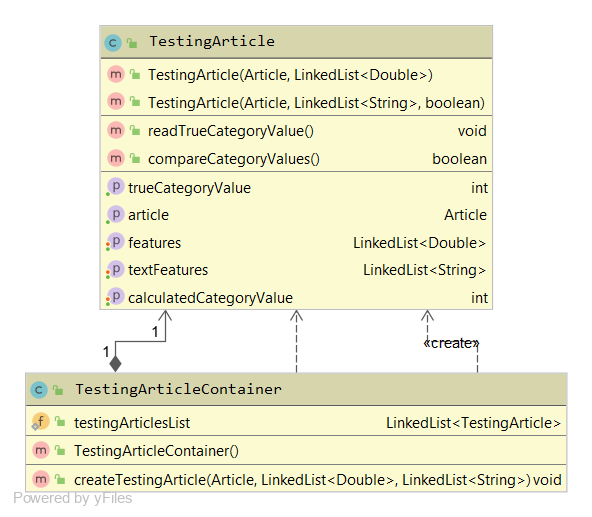
\includegraphics[width=1\textwidth]{{Diagramy/PackageTesting.png}}
	\caption{Diagram UML dla podpakietu $Testing$ pakietu $Model$}
\end{figure}

\subsection{Pakiet Features}
Pakiet $Features$ zawiera klasy służące do ekstrahowania cech. Wszystkie klasy pakietu $Features$ implementują interfejs $Feature$. \newline

Klasy pakietu $Features$ są następujące:
\begin{itemize}[label=$\bullet$\scshape\bfseries]
\item $Feature$ - interfejs implementowany przez wszystkie cechy,
\item $KeyWordsInBodyFeature$ - klasa ekstrahująca cechę $C_{1}$.
\item $KeyWordsInTitleFeature$ - klasa ekstrahująca cechę $C_{2}$.
\item $KeyWordsInDatelineFeature$ - klasa ekstrahująca cechę $C_{3}$.
\item $KeyWordsToAllWordsRatioFeature$ - klasa ekstrahująca cechę $C_{4}$.
\item $KeyWordsInFirst50WordsFeature$ - klasa ekstrahująca cechę $C_{5}$.
\item $KeyWordsInFirst10PerCentWordsFeature$ - klasa ekstrahująca cechę $C_{6}$.
\item $KeyWordsInFirst20PerCentWordsFeature$ - klasa ekstrahująca cechę $C_{7}$.
\item $KeyWordsInFirst50PerCentWordsFeature$ - klasa ekstrahująca cechę $C_{8}$.
\item $KeyWordsInFirstParagraphFeature$ - klasa ekstrahująca cechę $C_{9}$.
\item $KeyWordsInLast50WordsFeature$ - klasa ekstrahująca cechę $C_{10}$.
\item $KeyWordsInLast10PerCentWordsFeature$ - klasa ekstrahująca cechę $C_{11}$.
\item $KeyWordsInLastParagraphFeature$ - klasa ekstrahująca cechę $C_{12}$.\newline
\end{itemize}

\begin{figure}[H]
	\centering
	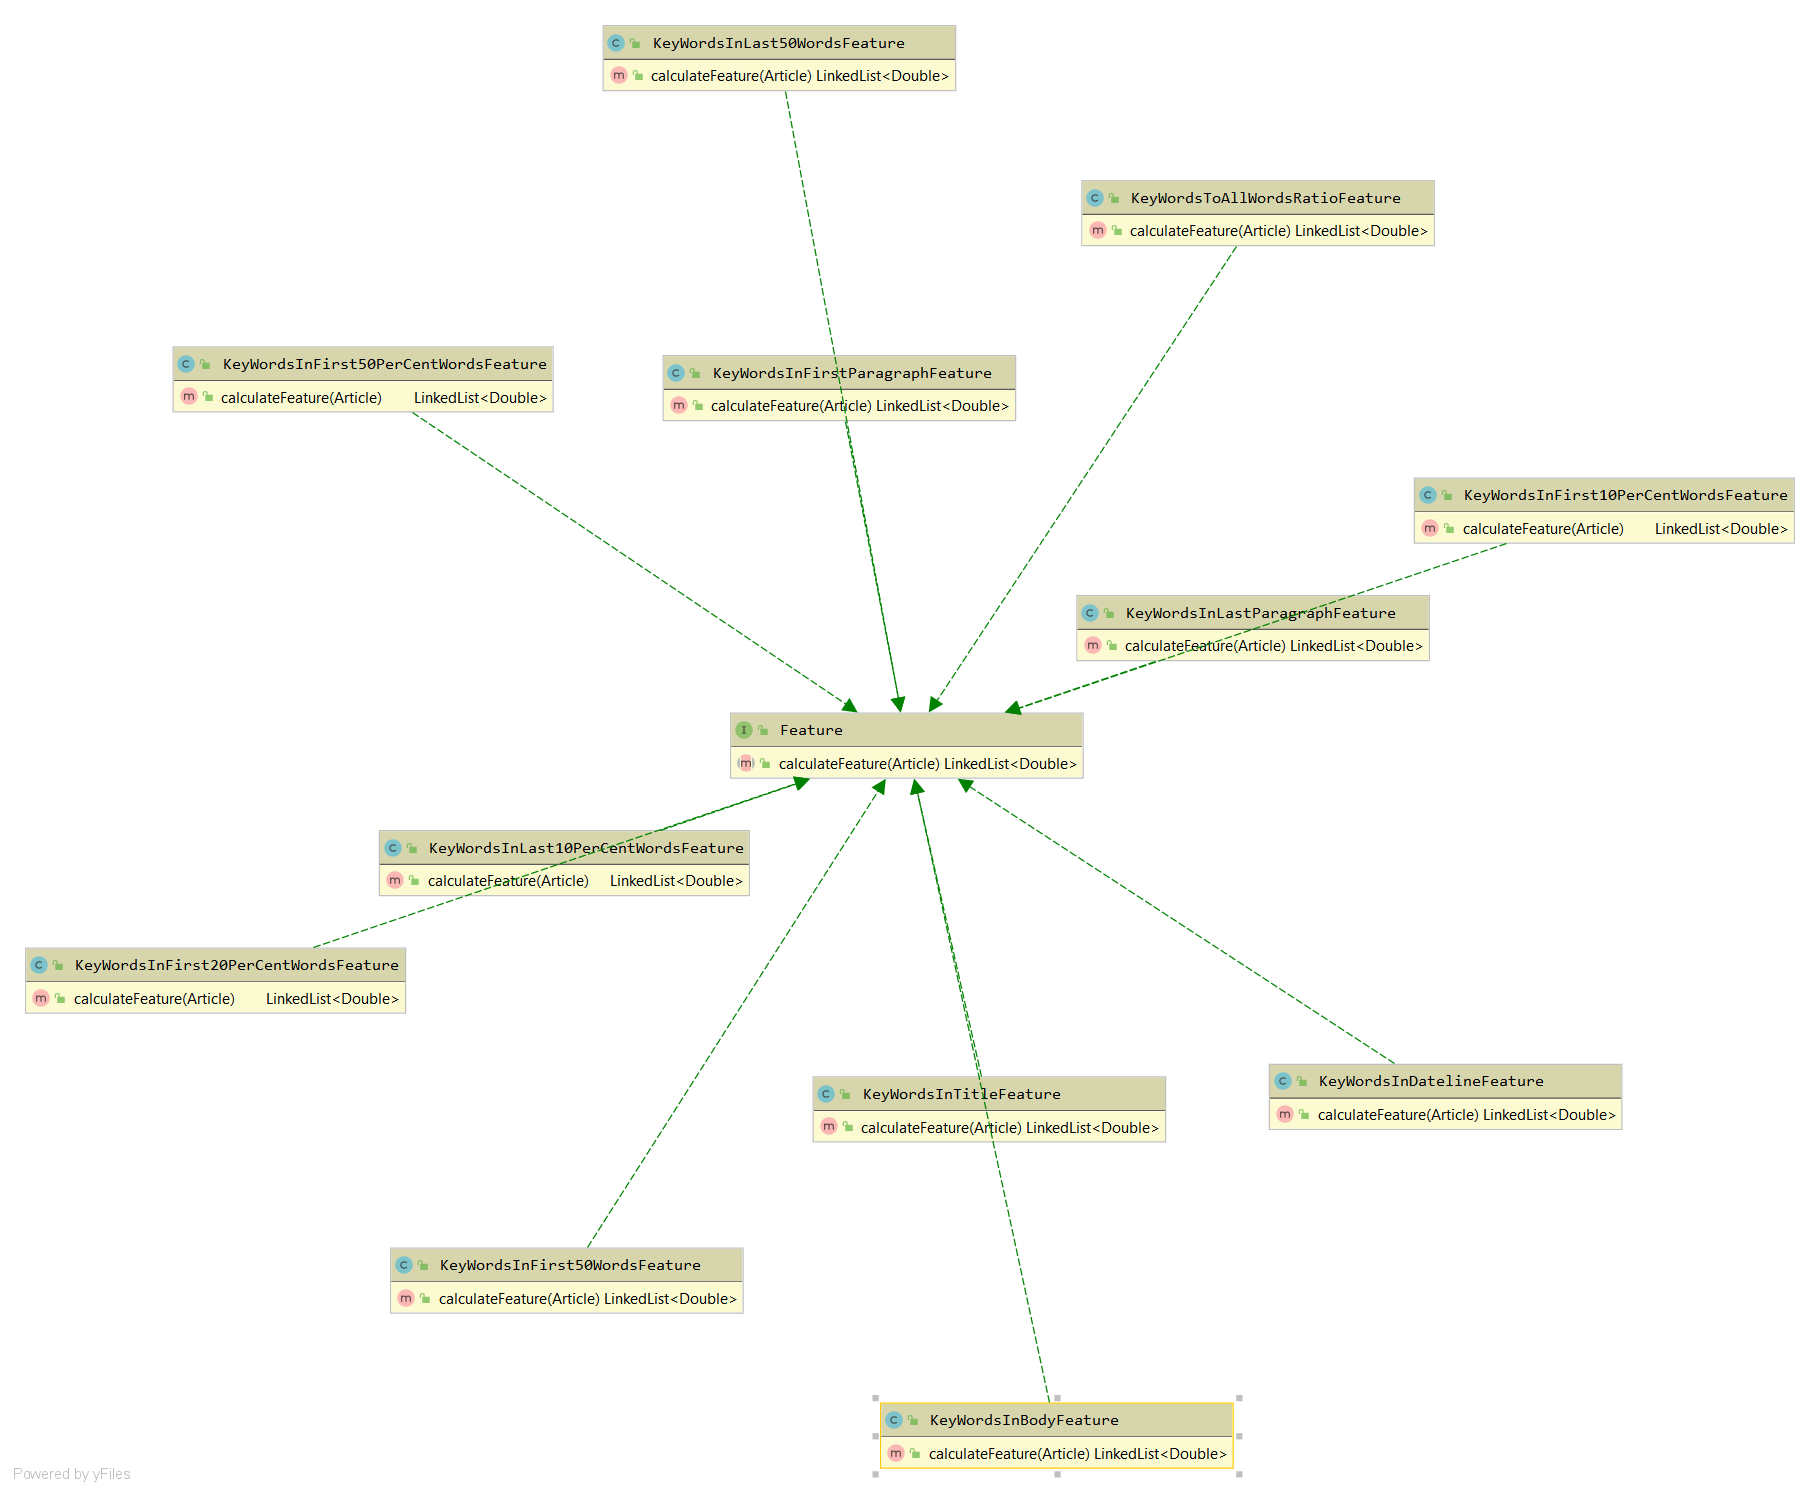
\includegraphics[width=1\textwidth]{{Diagramy/PackageFeatures.png}}
	\caption{Diagram UML dla pakietu $Features$}
\end{figure}

\subsection{Pakiet Calculations}
Pakiet $Calculations$ jest odpowiedzialny za wszelkiego rodzaju obliczenia. Zawiera on cztery podpakiety - $KeyWords$, $Features$, $KNN$ oraz $Metrics$.\newline

\begin{figure}[H]
	\centering
	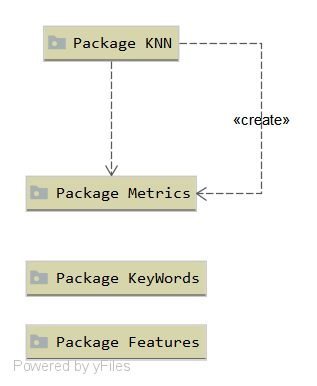
\includegraphics[width=0.4\textwidth]{{Diagramy/PackageCalculations.png}}
	\caption{Diagram podpakietów pakietu $Calculations$}
\end{figure}

\subsubsection{Podpakiet KeyWords}
Podpakiet $KeyWords$ odpowiada za wyznaczenie słów kluczowych. Klasy omawianego podpakietu implementują algorytm wyznaczania zwykłych jak i ważonych słów kluczowych, który został opisany we wcześniejszych rozdziałach.

\begin{figure}[H]
	\centering
	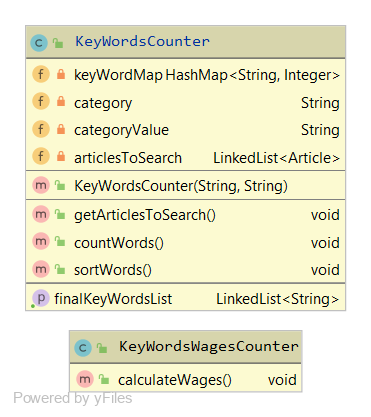
\includegraphics[width=0.6\textwidth]{{Diagramy/PackageCalculationsKeyWords.png}}
	\caption{Diagram UML dla podpakietu $KeyWords$ pakietu $Calculations$}
\end{figure}

Podpakiet $KeyWords$ zawiera dwie klasy:
\begin{itemize}[label=$\bullet$\scshape\bfseries]
\item $KeyWordsCounter$ - klasa implementująca algorytm wyznaczania słów kluczowych,
\item $KeyWordsWagesCounter$ - klasa służąca do obliczania wag słów kluczowych.\newline
\end{itemize}

\subsubsection{Podpakiet Features}
Podpakiet $Features$ pakietu $Calculations$ ma dwa główne zadania - przeprowadzenie ekstrakcji cech dla wszystkich artykułów, a następnie normalizację otrzymanych wektorów cech.\newline

Podpakiet $Features$ składa się z dwóch klas:
\begin{itemize}[label=$\bullet$\scshape\bfseries]
\item $FeaturesExtractor$ - klasa odpowiedzialna za przeprowadzenie procesu ekstrakcji cech kolejno dla wszystkich wczytanych artykułów,
\item $FeaturesNormaliser$ - klasa służąca do normalizacji otrzymanych wektorów cech.\newline
\end{itemize}

\begin{figure}[H]
	\centering
	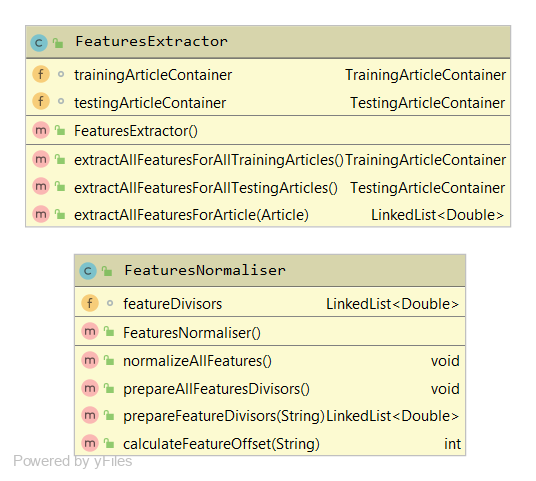
\includegraphics[width=0.8\textwidth]{{Diagramy/PackageCalculationsFeatures.png}}
	\caption{Diagram UML dla podpakietu $Features$ pakietu $Calculations$}
\end{figure}

\subsubsection{Podpakiet KNN}
Podpakiet $KNN$ implementuje omówiony we wprowadzeniu algorytm k najbliższych sąsiadów. Najlepsza kategoria wyznaczana jest dla wszystkich artykułów testowych.

\begin{figure}[H]
	\centering
	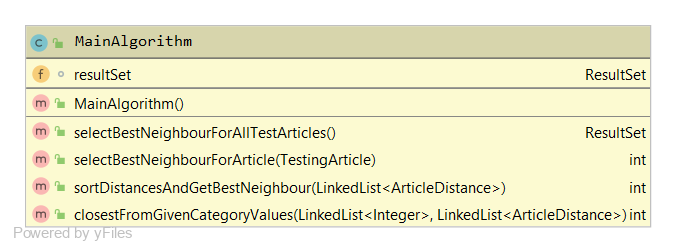
\includegraphics[width=1\textwidth]{{Diagramy/PackageCalculationsKNN.png}}
	\caption{Diagram UML dla podpakietu $KNN$ pakietu $Calculations$}
\end{figure}

Podpakiet $KNN$ składa się z jednej klasy - $MainAlgorithm$, odpowiedzialnej za przeprowadzenie klasyfikacji dla wszystkich artykułów testowych.\newline

\subsubsection{Podpakiet Metrics}
Podpakiet $Metrics$ zawiera implementacje wszystkich metryk omówionych we wprowadzeniu. Każda z pięciu metryk implementuje interfejs $Metrics$.\newline

\begin{figure}[H]
	\centering
	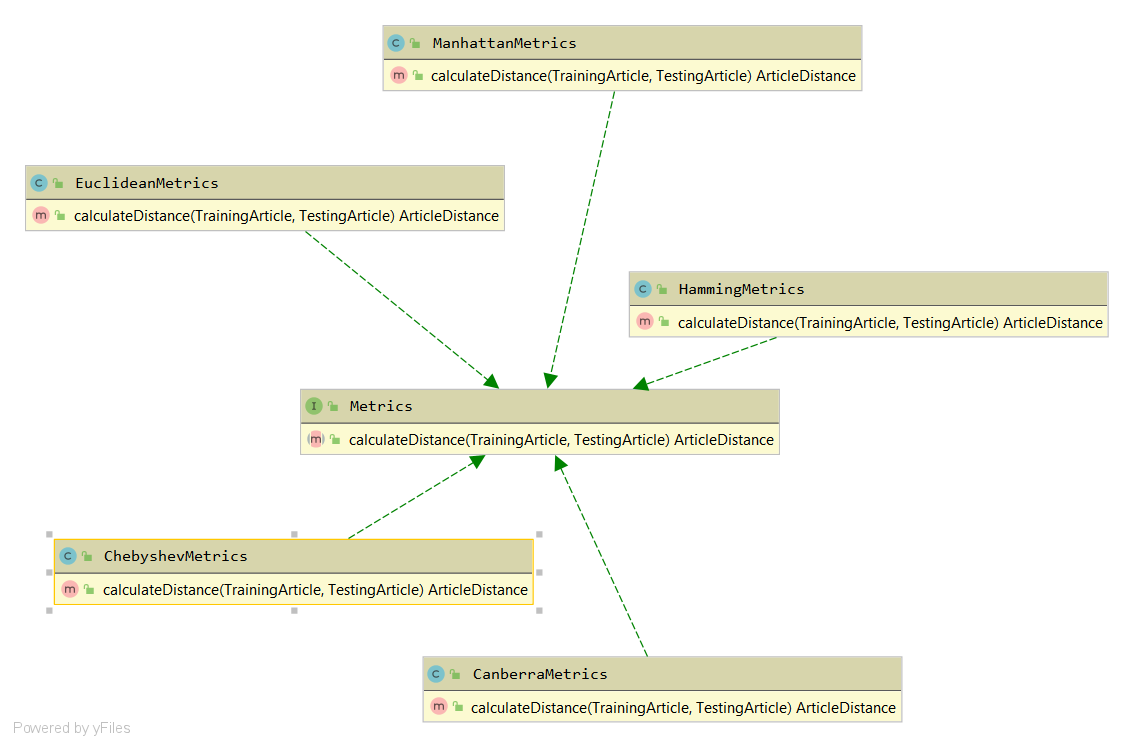
\includegraphics[width=1\textwidth]{{Diagramy/PackageCalculationsMetrics.png}}
	\caption{Diagram UML dla podpakietu $Metrics$ pakietu $Calculations$}
\end{figure}

Podpakiet $Metrics$ zawiera następujące klasy:
\begin{itemize}[label=$\bullet$\scshape\bfseries]
\item $Metrics$ - interfejs implementowany przez wszystkie metryki,
\item $EuclideanMetrics$ - klasa implementująca metrykę Euklidesową,
\item $ManhattanMetrics$ - klasa implementująca metrykę uliczną,
\item $ChebyshevMetrics$ - klasa implementująca metrykę Czebyszewa,
\item $HammingMetrics$ - klasa implementująca metrykę Hamminga,
\item $CanberraMetrics$ - klasa implementująca metrykę Canberra.
\end{itemize}

\subsection{Pakiet Main}
Pakiet $Main$ jest pakietem głównym, odpowiedzialnym za uruchomienie aplikacji, koordynowanie jej działania oraz określenie konfiguracji w jakiej aplikacja ma działać.\newline

\begin{figure}[H]
	\centering
	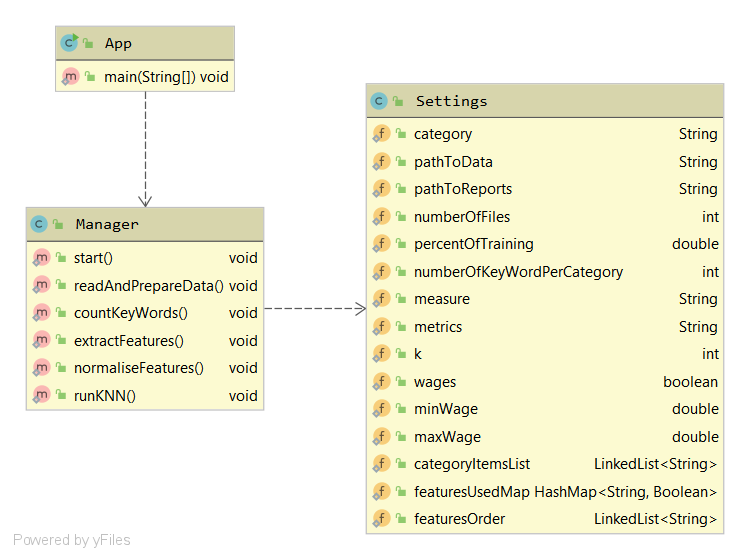
\includegraphics[width=1\textwidth]{{Diagramy/PackageMain.png}}
	\caption{Diagram UML dla pakietu $Main$}
\end{figure}

Pakiet $Main$ zawiera trzy klasy:
\begin{itemize}[label=$\bullet$\scshape\bfseries]
\item $App$ - klasa uruchamiająca program, wywołuje metodę $start()$ w klasie $Manager$,
\item $Manager$ - klasa sterująca kolejnością wywołania kolejnych modułów aplikacji,
\item $Settings$ - klasa ustawień, pozwalająca na ustawienie takich parametrów konfiguracyjnych jak metryka, wartość $k$ czy podział artykułów na treningowe i testowe.
\end{itemize}

\section{Materiały i metody}
W tym rozdziale omówione zostaną poszczególne eksperymenty jakie wykonano z użyciem naszego programu. \newline

Klasyfikacje artykułów przeprowadzano ze względu na dwa różne rodzaje etykiet. Pierwszym z nich była lokalizacja (place). Kategorie (etykiety) jakie wyróżniliśmy były następujące: west-germany, usa, france, uk, canada, japan. Klasyfikacja przeprowadzana była jedynie z wykorzystaniem artykułów, których pole "places" przyjmowało jedną z powyższych wartości. \newline

Drugim rodzajem etykiet był temat (topic). Kategorie (etykiety) jakie wyróżniliśmy były następujące: earn, trade, money-supply, acq. Podobnie jak w pierwszym przypadku, klasyfikacja przeprowadzana była jedynie z wykorzystaniem artykułów, których pole "topics" przyjmowało jedną z powyższych wartości.

\subsection{Wpływ liczby k sąsiadów oraz wyboru metryki na klasyfikację}
Klasyfikacja tekstów została wykonana z wykorzystaniem zbioru (zwykłych) słów kluczowych. Eksperymenty wykonano z użyciem wszystkich pięciu metryk. Dla każdego przypadku testowego dokonano klasyfikacji tekstu dla następujących wartości współczynnika k:
\begin{equation}
            k \in \{1, 3, 4, 6, 8, 10, 12, 14, 17, 20\}.
 \end{equation}
W każdym przypadku testowym zbiór treningowy stanowił 70\% artykułów, zaś zbiór testowy 30\% artykułów.

\subsection{Wpływ podziału tekstów na zbiory treningowe i testowe na klasyfikację}
Klasyfikacja tekstów została wykonana z wykorzystaniem zbioru (zwykłych) słów kluczowych. Eksperymenty przeprowadzono posługując się metryką Euklidesową. Wartość parametru k była stała i wynosiła $k=6$. Przeprowadzono klasyfikacje dla pięciu różnych podziałów artykułów na zbiory testowe i treningowe: 
\begin{itemize}[label=$\bullet$\scshape\bfseries]

\item Zbiór treningowy: 40\% artykułów, zbiór testowy 60\%,
\item Zbiór treningowy: 50\% artykułów, zbiór testowy 50\%,
\item Zbiór treningowy: 60\% artykułów, zbiór testowy 40\%,
\item Zbiór treningowy: 70\% artykułów, zbiór testowy 60\%,
\item Zbiór treningowy: 80\% artykułów, zbiór testowy 20\%.

\end{itemize}

\subsection{Wpływ konkretnych cech na klasyfikację}
Klasyfikacja tekstów została wykonana z wykorzystaniem zbioru (zwykłych) słów kluczowych. Eksperymenty przeprowadzono posługując się metryką Euklidesową. Wartość parametru k była stała i wynosiła $k=6$. W każdej iteracji programu zbiór treningowy stanowił 70\% artykułów, zaś zbiór testowy 30\% artykułów. Przeprowadzono klasyfikacje dla czterech różnych zestawów cech, wybranych spośród wszystkich cech omówionych w rozdziale 2.4. Wybrane zestawy cech były następujące (aby nie duplikować treści, w tym miejscu posługuję się indeksami funkcji cech z rodziału 2.4):
\begin{itemize}[label=$\bullet$\scshape\bfseries]

\item Zestaw 1: $C_{1}$,  $C_{2}$,  $C_{3}$,  $C_{4}$,  $C_{10}$,  $C_{11}$,  $C_{12}$,
\item Zestaw 2: $C_{1}$,  $C_{2}$,  $C_{3}$,  $C_{4}$,
\item Zestaw 2: $C_{5}$,  $C_{6}$,  $C_{7}$,  $C_{8}$,  $C_{9}$,
\item Zestaw 2: $C_{2}$,  $C_{3}$,  $C_{6}$,  $C_{11}$.
\end{itemize}

\subsection{Wpływ użycia ważonych słów kluczowych na klasyfikację}
Klasyfikacja tekstów została wykonana z wykorzystaniem zbioru zwykłych oraz z użyciem ważonych słów kluczowych. Eksperymenty wykonano z użyciem wszystkich pięciu metryk. Wartość parametru k była stała i wynosiła $k=6$. W każdym przypadku testowym zbiór treningowy stanowił 70\% artykułów, zaś zbiór testowy 30\% artykułów.

\section{Wyniki}
W tym rozdziale zamieszczono tabele oraz wykresy prezentujące wyniki przeprowadzanych przez nas eksperymentów.

\subsection{Wpływ liczby k sąsiadów oraz wyboru metryki na klasyfikację}

\begin{table}[H]
	\centering
	\begin{tabular}{c c c c} 
		\hline
		\textbf{k} & \textbf{places [\%]} & \textbf{topics [\%]} \\ [0.5ex] 
		\hline
		\hline 
1	& 81,99 &	91,35 \\
3	& 84,99 &	95,06 \\
4	& 85,41 & 94,69 \\
6	& 85,79 &	96,23 \\
8	&85,14 &	95,97 \\
10	&85,07&	94,90 \\
12	&85,34&	95,49 \\
14	&85,19&	95,38 \\
17	&85,07&	95,49 \\
20	&85,04&	95,70 \\
		\hline
	\end{tabular}
	\caption{Skuteczność klasyfikacji dla metryki Euklidesowej}
\end{table}

\begin{table}[H]
	\centering
	\begin{tabular}{c c c c} 
		\hline
		\textbf{k} & \textbf{places [\%]} & \textbf{topics [\%]} \\ [0.5ex] 
		\hline
		\hline 
1	&	81,64	&	86,25	\\
3	&	84,92	&	88,06	\\
4	&	85,36	&	87,74	\\
6	&	85,86	&	88,91	\\
8	&	84,35	&	88,75	\\
10	&	84,27	&	88,96	\\
12	&	84,35	&	89,28	\\
14	&	84,35	&	87,58	\\
17	&	84,20	&	87,53	\\
20	&	84,12	&	87,05	\\
		\hline
	\end{tabular}
	\caption{Skuteczność klasyfikacji dla metryki Chebysheva}
\end{table}

\begin{table}[H]
	\centering
	\begin{tabular}{c c c c} 
		\hline
		\textbf{k} & \textbf{places [\%]} & \textbf{topics [\%]} \\ [0.5ex] 
		\hline
		\hline 
1	&	82,15	&	94,64	\\
3	&	86,26	&	96,66	\\
4	&	86,26	&	96,76	\\
6	&	87,00	&	97,03	\\
8	&	87,10	&	96,97	\\
10	&	86,93	&	96,92	\\
12	&	86,78	&	97,03	\\
14	&	86,75	&	96,82	\\
17	&	86,28	&	96,82	\\
20	&	86,08	&	96,60	\\
		\hline
	\end{tabular}
	\caption{Skuteczność klasyfikacji dla metryki ulicznej}
\end{table}

\begin{table}[H]
	\centering
	\begin{tabular}{c c c c} 
		\hline
		\textbf{k} & \textbf{places [\%]} & \textbf{topics [\%]} \\ [0.5ex] 
		\hline
		\hline 
1	&	79,46	&	92,20	\\
3	&	82,09	&	94,11	\\
4	&	82,63	&	93,79	\\
6	&	82,96	&	93,90	\\
8	&	82,91	&	94,32	\\
10	&	83,03	&	94,11	\\
12	&	82,96	&	94,00	\\
14	&	82,86	&	94,00	\\
17	&	82,71	&	94,00	\\
20	&	82,66	&	94,16	\\
		\hline
	\end{tabular}
	\caption{Skuteczność klasyfikacji dla metryki Hamminga}
\end{table}

\begin{table}[H]
	\centering
	\begin{tabular}{c c c c} 
		\hline
		\textbf{k} & \textbf{places [\%]} & \textbf{topics [\%]} \\ [0.5ex] 
		\hline
		\hline 
1	&	81,10	&	95,01	\\
3	&	84,12	&	96,28	\\
4	&	84,25	&	96,02	\\
6	&	84,74	&	96,39	\\
8	&	84,79	&	96,71	\\
10	&	84,62	&	96,71	\\
12	&	84,59	&	96,71	\\
14	&	84,64	&	96,76	\\
17	&	84,30	&	96,60	\\
20	&	84,25	&	96,76	\\
		\hline
	\end{tabular}
	\caption{Skuteczność klasyfikacji dla metryki Canberra}
\end{table}

\begin{figure}[H]
	\centering
	\includegraphics[width=1\textwidth]{{Wykresy/places10k.png}}
	\caption{Wizualizacja danych z Tabel 1-5 dla kategorii "places"}
\end{figure}

\begin{figure}[H]
	\centering
	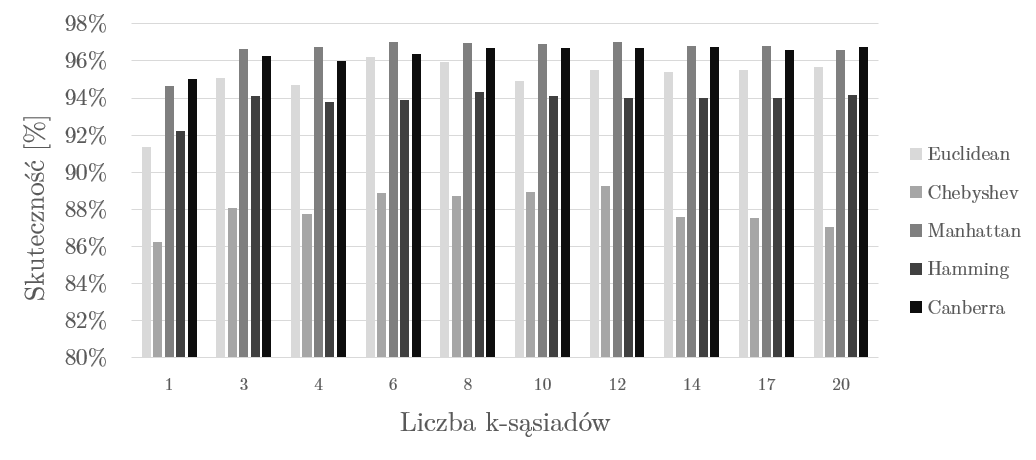
\includegraphics[width=1\textwidth]{{Wykresy/topics10k.png}}
	\caption{Wizualizacja danych z Tabel 1-5 dla kategorii "topics"}
\end{figure}

\subsection{Wpływ podziału tekstów na zbiory treningowe i testowe na klasyfikację}

\begin{table}[H]
	\centering
	\begin{tabular}{c c c c} 
		\hline
		\textbf{Podział} & \textbf{places [\%]} & \textbf{topics [\%]} \\ [0.5ex] 
		\hline
		\hline 
40:60	&	87,04	&	93,89	\\
50:50	&	86,09	&	94,52	\\
60:40	&	85,69	&	94,71	\\
70:30	&	85,79	&	96,23	\\
80:20	&	84,78	&	96,74	\\

		\hline
	\end{tabular}
	\caption{Skuteczność klasyfikacji dla różnych podziałów artykułów (podano w kolejności treningowe:testowe)}
\end{table}

\begin{figure}[H]
	\centering
	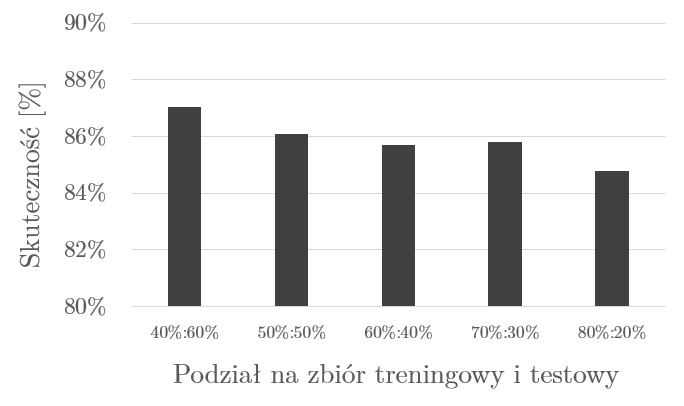
\includegraphics[width=0.8\textwidth]{{Wykresy/podzial_places.png}}
	\caption{Wziualizacja danych z Tabeli 6 dla kategorii "places"}
\end{figure}

\begin{figure}[H]
	\centering
	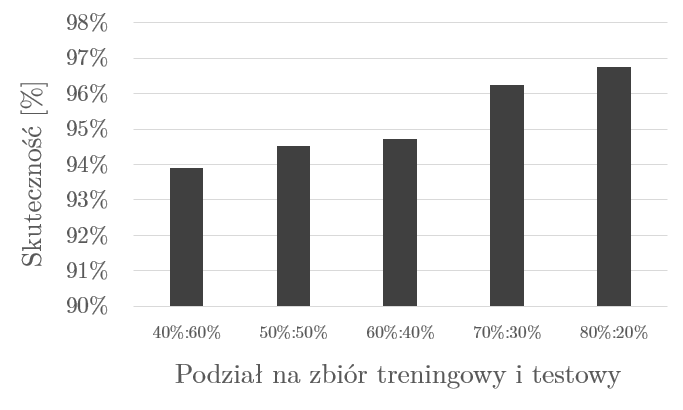
\includegraphics[width=0.8\textwidth]{{Wykresy/podzial_topics.png}}
	\caption{Wizualizacja danych z Tabeli 6 dla kategorii "topics"}
\end{figure}

\subsection{Wpływ konkretnych cech na klasyfikację}

\begin{table}[H]
	\centering
	\begin{tabular}{c c c c} 
		\hline
		\textbf{Zestaw} & \textbf{places [\%]} & \textbf{topics [\%]} \\ [0.5ex] 
		\hline
		\hline 
1	&	85,19	&	95,91 \\
2	&	84,32	&	95,38 \\
3	&	85,14	&	96,18 \\
4	&	79,61	&	79,41 \\

		\hline
	\end{tabular}
	\caption{Skuteczność klasyfikacji dla różnych zestawów cech}
\end{table}

\begin{figure}[H]
	\centering
	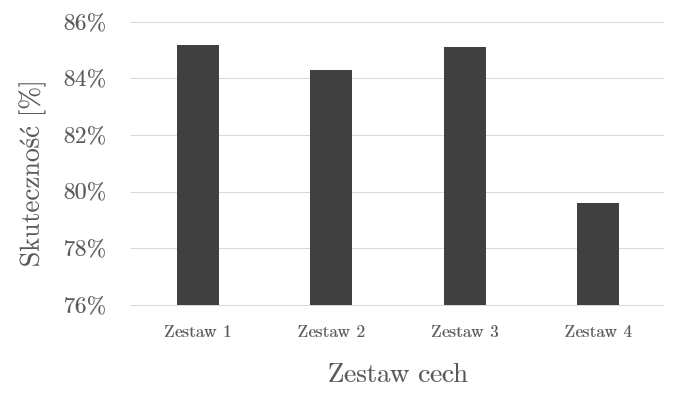
\includegraphics[width=0.8\textwidth]{{Wykresy/cechy_places.png}}
	\caption{Wizualizacja danych z Tabeli 7 dla kategorii "places"}
\end{figure}

\begin{figure}[H]
	\centering
	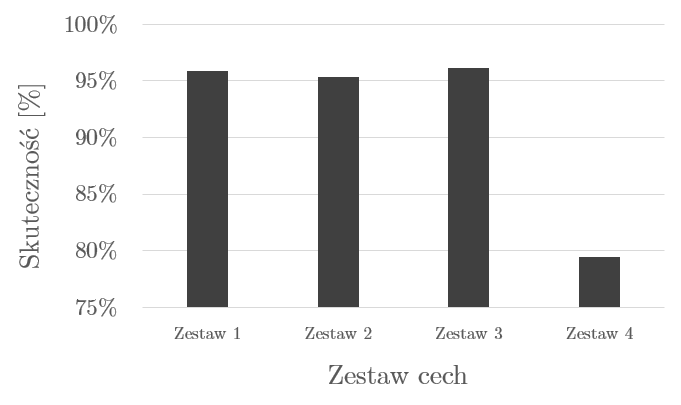
\includegraphics[width=0.8\textwidth]{{Wykresy/cechy_topics.png}}
	\caption{Wizualizacja danych z Tabeli 7 dla kategorii "topics"}
\end{figure}

\subsection{Wpływ użycia ważonych słów kluczowych na klasyfikację}
\begin{table}[H]
	\centering
	\begin{tabular}{c c c c} 
		\hline
		\textbf{Metryka} & \textbf{zwykłe słowa kluczowe [\%]} & \textbf{ważone słowa klczuowe [\%]} \\ [0.5ex] 
		\hline
		\hline 
Euclidean	&	85,79	&	88,54	\\
Chebyshev	&	85,86	&	88,17	\\
Manhattan	&	87,00	&	88,32	\\
Hamming	&	82,96	&	83,03	\\
Canberra	&	84,74	&	86,68	\\
		\hline
	\end{tabular}
	\caption{Skuteczność klasyfikacji dla różnych metod ekstrakcji - zywkłe i ważone słowa kluczowe - kategoria "places"}
\end{table}

\begin{table}[H]
	\centering
	\begin{tabular}{c c c} 
		\hline
		\textbf{Metryka} & \textbf{zwykłe słowa kluczowe [\%]} & \textbf{ważone słowa klczuowe [\%]} \\ [0.5ex] 
		\hline
		\hline 
Euclidean	&	96,23	&	96,50	\\
Chebyshev	&	88,91	&	93,68	\\
Manhattan	&	97,03	&	96,92	\\
Hamming	&	93,90	&	94,37	\\
Canberra	&	96,39	&	96,60	\\
		\hline
	\end{tabular}
	\caption{Skuteczność klasyfikacji dla różnych metod ekstrakcji - zywkłe i ważone słowa kluczowe - kategoria "topics"}
\end{table}

\begin{figure}[H]
	\centering
	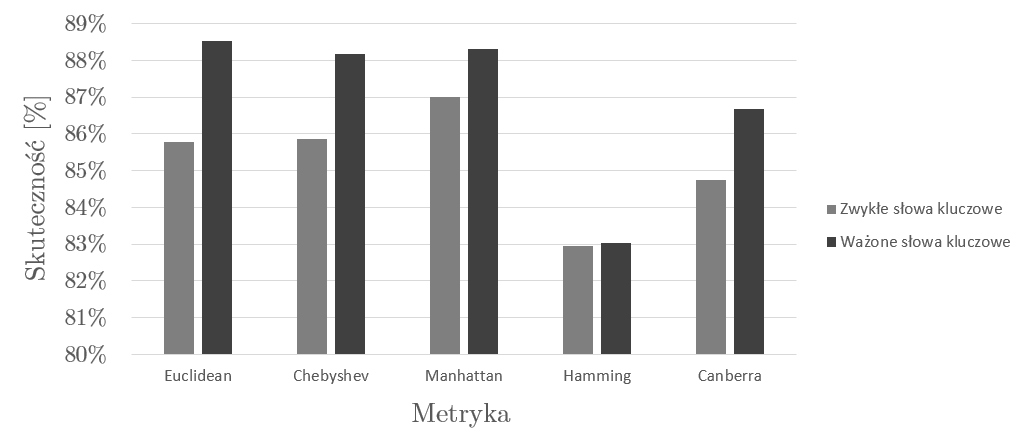
\includegraphics[width=1\textwidth]{{Wykresy/wazone_places.png}}
	\caption{Wizualizacja danych z Tabeli 8}
\end{figure}

\begin{figure}[H]
	\centering
	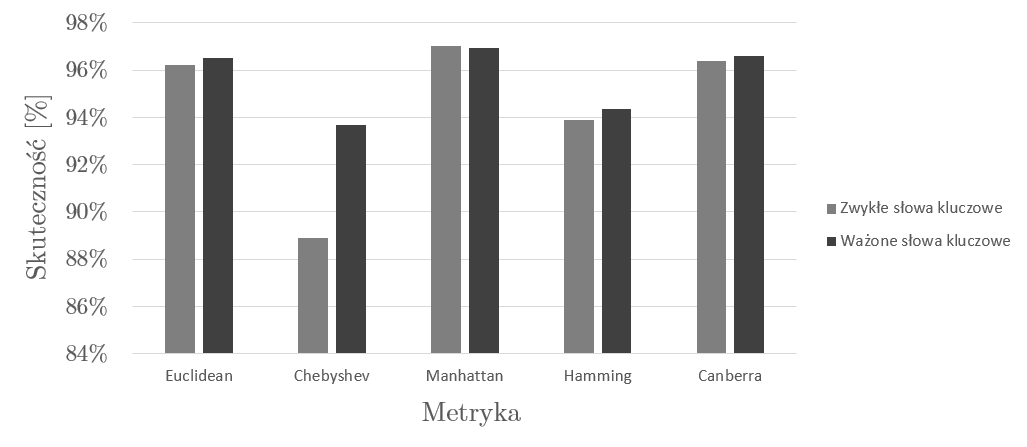
\includegraphics[width=1\textwidth]{{Wykresy/wazone_topics.png}}
	\caption{Wizualizacja danych z Tabeli 9}
\end{figure}
\section{Dyskusja}
$ Praca\ w\ toku $

\section{Wnioski}
$ Praca\ w\ toku $

\begin{thebibliography}{4}
\bibitem{wyklad} 
A. Niewiadomski
\textit{Materiały, przykłady i ćwiczenia do przedmiotu Komputerowe Systemy Rozpoznawania}. 
19 czerwca 2012.
\bibitem{Maven} 
Narzędzie Maven
\textit{https://maven.apache.org/}. 
\bibitem{Stem} 
Bibliotek snowball-stemmer
\textit{https://mvnrepository.com/artifact/com.github.rholder/snowball-stemmer}. 
\bibitem{Excel} 
Biblioteka poi-ooxml
\textit{https://mvnrepository.com/artifact/org.apache.poi/poi-ooxml}. 
\end{thebibliography}

\end{document}
